\documentclass[handout, 8pt]{beamer}

%\usetheme{Warsaw}

\usepackage{pgfpages}
\usepackage{graphicx}
\usepackage{amsmath}
\usepackage{amsfonts}
\usepackage{amssymb}
\usefonttheme{serif}

\usepackage{mathtext}


\usepackage[T2A]{fontenc}
\usepackage[utf8]{inputenc}
\usepackage[english,ukrainian]{babel} 

\numberwithin{figure}{section}
\numberwithin{equation}{section}
\numberwithin{table}{section}
\setbeamertemplate{caption}[numbered]

\usepackage[justification=centering]{caption}
%\setbeamersize{text margin left=5pt,text margin right=5pt}

\pgfpagesuselayout{2 on 1}[a4paper, border shrink=2mm]

\title{Амплiтудно-частотнi характеристики шаруватих пластин i гофрованих цилiндричних оболонок}
\author[Горячко Тарас Всеволодович]{{\large Горячко Тарас Всеволодович}\\[10mm]{\small Науковий керівник: доктор фізико-математичних наук, професор\\ Марчук М.В. }}
\institute{Інститут прикладних проблем механіки і математики ім. Я.С.~Підстригача \\ НАН України\\[\medskipamount]
      
\includegraphics[width=0.25\textwidth,height=0.2\textheight]{pic/ilogo.jpg}%
}
\date{}

\begin{document}
\begin{frame}
\titlepage
\end{frame}
\setbeamertemplate{footline}[frame number]

\begin{frame}{Вступ}
\begin{block}{Мета дисертаційної роботи}
Розвиток методу збурень в поєднанні з методом скінченних елементів стосовно задач визначення амплітудно-частотних характеристик шаруватих пластин і гофрованих цилiндричних оболонок за лінійних та геометрично нелінійних коливань.
\end{block}
\begin{block}{Об’єкт дослідження}
Процеси лінійних і геометрично нелінійних коливань шаруватих пластин i гофрованих цилiндричних оболонок.
\end{block}
\begin{block}{Предмет дослідження}
Спектри власних частот та амплітудно-частотні залежності шаруватих пластин i гофрованих цилiндричних оболонок за лінійних та геометрично нелінійних коливань.
\end{block}

\begin{block}{Публікації та апробації за темою дисертації}
За результатами досліджень опубліковано 17 наукових робіт, із них 2 статті у журналі, який реферується наукометричною базою Scopus:
\begin{enumerate}
\item Marchuk M., Goriachko T., Pakosh V. Geometrically Nonlinear Free Transversal Vibrations of Thin-Walled Elongated Panels with Arbitrary Generatrix // Vibrations in Physical Systems. – 2014. – Vol. 26. – P. 153–160.
\item Marchuk M., Goriachko T., Pakosh V. Natural Frequencies of Layered Elongated Cylindrical Panels for Geometrically Nonlinear Deformation at Discrete Consideration of Components // Vibrations in Physical Systems. – 2016. – Vol. 27. – P. 255–264.
\end{enumerate}

\end{block}

\end{frame}


\section{Розділ 1}

\begin{frame}{Розділ 1. Огляд публікацій за проблемою визначення  амплітудно-частотних характеристик шаруватих пластин і гофрованих циліндричних оболонок за лінійного та геометрично нелінійного деформування}


%\medskip Дослідження напружено-деформованого стану тонкостінних елементів конструкцій на основі уточнених теорій відображені в роботах С.~О.~Амбарцумяна, В.~З.~Власова, Й.~І.~Воровича, К.~З.~Галімова, О.~Л.~Гольденвейзера, Я.~М.~Григоренка, О.~М.~Гузя, Л.~Донелла, Р.~Міндліна, П.~Нагді, Е.~Рейснера, С.~П.~Тимошенка та інших учених.

\medskip
Постановкам задач про геометрично нелінійні коливання пластин і оболонок та розробці методів їх розв'язання присвячені праці Н.~А.~Алумяе,  О.~І.~Беспалової, В.~В.~Болотіна, В.~Є.~Вериженка, А.~С.~Вольміра, В.~Т.~Грінченка, Е.~І.~Григолюка, О.~Я.~Григоренка, Я.~М.~Григоренка, Я.~О.~Жука, Б.~Я.~Кантора, Я.~Ф.~Каюка, М.~С.~Корнішина, В.~А.~Криська, Л.~В.~Курпи, Р.~М.~Кушніра, М.~В.~Марчука, А.П. Мукоєда, С.~П.~Тимошенка, І.~М.~Турчина, M.~Amabili, J.~Awrejcewicz, I.~K.~Banerjee, I.~C.~Chen, Li.~A.~Dong, C.~L.~Dym, P.~B.~Goncalves,  L.~Librescu, M.~Sundhakar, T.~Ueda та інших учених.

\medskip 
Розробці та розвиненню методу скінченних елементів для нелінійних задач присвячені роботи А.~С.~Городецького, І.~І.~Дияка, В.~Г.~Піскунова, В.~А.~Постнова, О.~О.~Рассказова, Л.~А.~Розіна, Р.~Б.~Рікардса, М.~В.~Марчука, І.~С.~Мухи, Я.~Г.~Савули, А.~С.~Сахарова, М.~М.~Шапошнікова, Г.~А.~Шинкаренка, K.-J.~Bathe, T.~Belytschko, M.~A.~Crisfield, R.~H.~Gallager, J.~N.~Reddy, J.~T.~Oden, G.~Streng, E.~L.~Wilson, O.~C.~Zienkiewicz та інших учених.

\medskip 
Застосуванню методу збурень для нелінійних задач стійкості і коливань присвячені роботи D.~A.~Evensen, A.~H.~Nayfeh and D.~T.~Mook, L.~W.~Rehfield, B.~Budiansky, J.~Wedel-Heinen, E.~L.~Jansen, T.~Rahman, R.~Lewandowski, E.~J.~Hinch та інших учених.


\end{frame}

%\begin{frame}{Розділ 1.}
%
%
%
%
%\medskip
%Дослідженню коливань гофрованих оболонок і пластин присвячені роботи Н.~П.~Семенюка, Г.~Р.~Гулгазаряна, Л.~Г.~Гулгазаряна, K.~M.~Liew, N.~K.~Mandal, G.~Kress, M.~Winkler та інших учених.
%
%\begin{block}{Мета дисертаційної роботи}
%Розвиток методу збурень в поєднанні з методом скінченних елементів стосовно задач визначення амплітудно-частотних характеристик шаруватих пластин і гофрованих цилiндричних оболонок за лінійних та геометрично нелінійних коливань.
%\end{block}
%
%
%\end{frame}

%\begin{frame}
%
%\textbf{Завдання}
%\\
%\vspace{1em}
%\begin{itemize}
%\item формулювання постановки початково-крайових та варіаційних задач про геометрично нелінійне динамічне деформування шаруватих пластин і гофрованих циліндричних оболонок;
%\item виведення деформаційних співвідношень для оболонок з довільною напрямною;
%\item узагальнення методу збурень для розв’язування системи нелінійних алгебраїчних рівнянь, який дає змогу позбутися секулярного члена у розв’язку задачі;
%\item створення на основі розроблених алгоритмів програмного забезпечення для розв’язування задач визначення амплітудно-частотних характеристик шаруватих пластин і гофрованих циліндричних оболонок за геометрично нелінійного деформування;
%\item розроблення методології проведення числових експериментів з метою встановлення достовірності запропонованого підходу;
%\item проведення розрахунків характеристик коливних процесів.
%
%\end{itemize}
%
%
%\end{frame}



\section{Розділ 2}

\begin{frame}{Розділ 2. РІВНЯННЯ ДИНАМІЧНО НАПРУЖЕНОГО СТАНУ ЗА ГЕОМЕТРИЧНО НЕЛІНІЙНОГО ДЕФОРМУВАННЯ}
\textbf{Співвідношення просторової геометрично нелінійної динамічної теорії пружності в криволінійній системі координат}
\begin{columns}
	\begin{column}{0.32\linewidth}
		\begin{figure}
			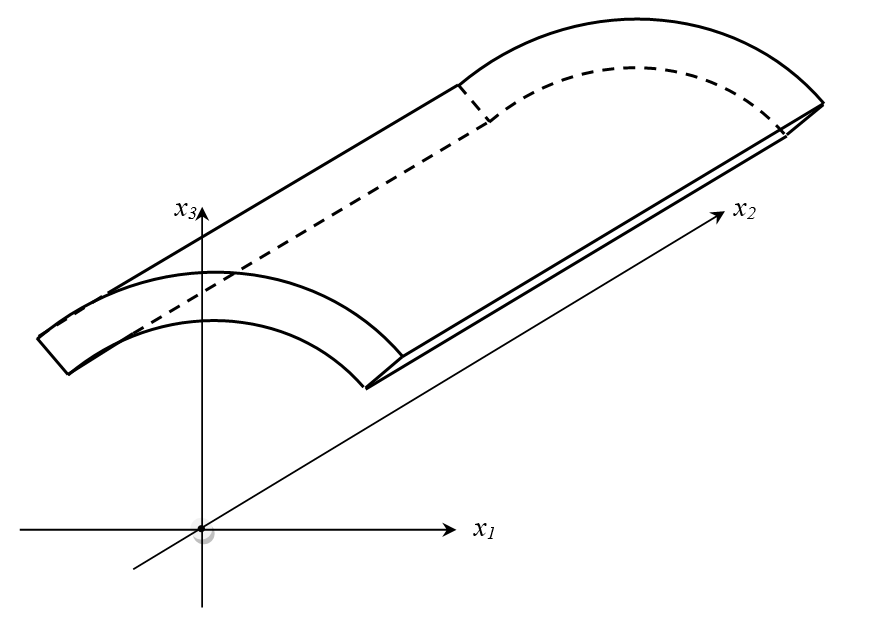
\includegraphics[scale=0.15]{pic/layer.png}
			\caption{ }
			\label{fig:21}
		\end{figure}
	\end{column}
	\begin{column}{0.68\textwidth}
Напружено-деформований стан описується $\vec{u}$, $\hat{\varepsilon}$, $\hat{\Sigma}$.
\begin{equation}
\varepsilon_{ij} = \frac{1}{2} \left( \nabla_i u_j + \nabla_j u_i + \nabla_i u^j \nabla_j u_k \right),
\end{equation}
\begin{equation}
\sigma^{ij} = C^{ijkm}\varepsilon_{km}.
\end{equation}
\emph{Рівняння руху}
\begin{equation} \label{eq:P}
div \hat{P} = \rho \frac{\partial^2 \vec{u}}{\partial t^2},
\end{equation}
де $\hat{P}$ --- перший несиметричний тензор Кірхгофа-Піоли, $\rho$ --- густина шару, $t$ --- час.
	\end{column}
\end{columns}
\begin{columns}
    \column{\dimexpr\paperwidth-40pt}
\emph{Граничні умови}
\begin{align}
&P^{3i}\left( \alpha_1, \alpha_2, \pm h/2, t \right) = X^{\pm}_{3i}\left( \alpha_1, \alpha_2, t \right),i=1,2,3, \alpha_1\in\left[\alpha_1^0;\alpha_1^1\right],\alpha_2\in\left[\alpha_2^0;\alpha_2^1\right]\\
&P^{im}\left( \alpha_1, \alpha_2, \alpha_3, t \right)n_i = f^{m}\left( \alpha_1, \alpha_2, \alpha_3, t \right), i,m=1,2,3, \left( \alpha_1, \alpha_2,\alpha_3\right)\in\Omega_{\sigma},\\
&u^{i}\left( \alpha_1, \alpha_2, \alpha_3, t \right) =g^{i}\left( \alpha_1, \alpha_2, \alpha_3, t \right), i=1,2,3, \left( \alpha_1, \alpha_2,\alpha_3\right)\in\Omega_{u}.
\end{align}
\emph{Початкові умови}
\begin{equation}
u^{i}\vline _{t=t_0} = u^i_0 \left( \alpha_1, \alpha_2, \alpha_3 \right), \frac{\partial u^{i}}{\partial t}\vline _{t=t_0} =v^i_0 \left( \alpha_1, \alpha_2, \alpha_3 \right), i=1,2,3.
\end{equation}
  \end{columns}
\end{frame}

\begin{frame}{Розділ 2}
\textbf{Побудова одновимірної моделі на основі двовимірної}
\\
\vspace{1pt}
Апроксимація переміщень $u_1$ та $u_3$, за координатою $\alpha_3$ 
\begin{align}
u_1 \left( \alpha_1, \alpha_3 \right) = u_{10} \left( \alpha_1\right)p_0 \left( \alpha_3\right)+u_{11} \left( \alpha_1\right)p_1 \left( \alpha_3\right)+u_{12} \left( \alpha_1\right)p_2 \left( \alpha_3\right),\\
u_3 \left( \alpha_1, \alpha_3 \right) = u_{30} \left( \alpha_1\right)p_0 \left( \alpha_3\right)+u_{31} \left( \alpha_1\right)p_1 \left( \alpha_3\right)+u_{32} \left( \alpha_1\right)p_2 \left( \alpha_3\right),
\end{align}
де поліноми $p_0$, $p_1$ та $p_2$ мають вигляд
\begin{equation}
p_0 \left( \alpha_3\right) = \frac12-\frac{\alpha_3}{h},
p_1 \left( \alpha_3\right) = \frac12+\frac{\alpha_3}{h},
p_2 \left( \alpha_3\right) = 1-\left(\frac{2\alpha_3}{h}\right)^2,
\end{equation}
$h$ --- товщина шару.
\begin{figure}
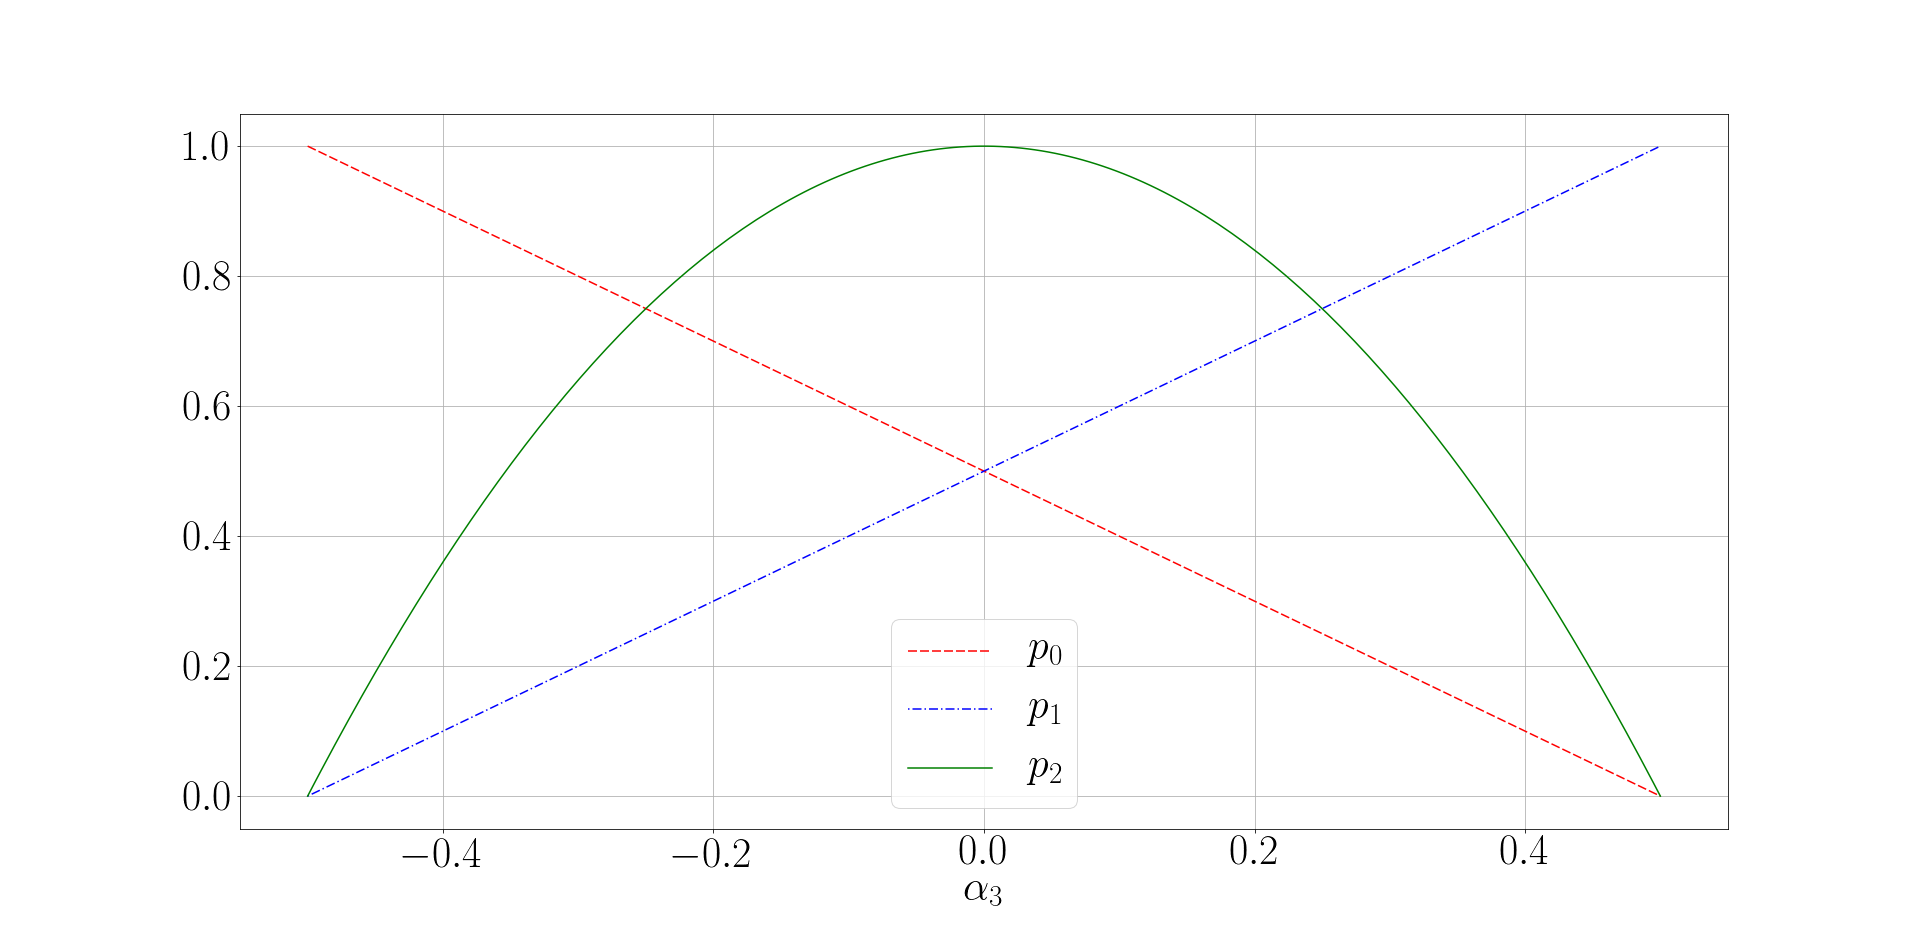
\includegraphics[scale=0.1]{pic/polin.png}
\caption{Графіки поліномів $p_0$, $p_1$ та $p_2$ на проміжку [-0.5;0.5]}
\end{figure}

\end{frame}

\begin{frame}{Розділ 2}
\begin{figure}
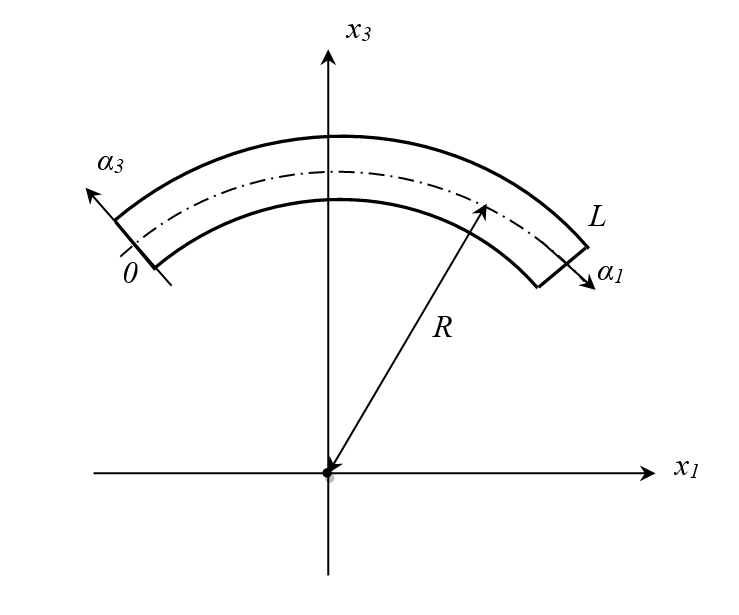
\includegraphics[scale=0.25]{pic/cylplate_2D.png}
\caption{Криволінійний пружний шар в декартовій системі координат.}
\end{figure}
\begin{equation}
\begin{aligned}
&\varepsilon_{ij} \left( \alpha_1, \alpha_3 \right) = \frac{\varepsilon_{ij0} \left( \alpha_1\right)p_0 \left( \alpha_3\right)+\varepsilon_{ij1} \left( \alpha_1\right)p_1 \left( \alpha_3\right)+\varepsilon_{ij2} \left( \alpha_1\right)p_2 \left( \alpha_3\right)}{1+\alpha_3 K\left( \alpha_1 \right)},\\
&\varepsilon_{ijk} = e_{ijk}\left( \alpha_1\right)+\eta_{ijk}\left( \alpha_1\right), \quad i,j=1,3, k=0,1,2,
\end{aligned}
\end{equation}

\begin{tabbing}
де \= $e_{ijk}\left( \alpha_1\right)$ --- лінійна складова,\\
\> $\eta_{ijk}\left( \alpha_1\right)$ --- нелінійна складова.
\end{tabbing}
\end{frame}

\begin{frame}{Розділ 2}
\begin{equation}\label{eq:sqt_strain_l}
\begin{aligned}
&e_{11k}\left(\alpha_1\right)=\frac{1}{A\left(\alpha_1\right)}\frac{du_{1k}}{d\alpha_1}+u_{3k}K\left(\alpha_1\right), k=0,1,2,
\\
&\begin{split}
e_{130}\left(\alpha_1\right)=u_{10}\left( -\frac{1}{h}-\frac{K\left( \alpha_1 \right)}{2} \right)+u_{11}\left( \frac{1}{h}-\frac{K\left( \alpha_1 \right)}{2} \right)+ \\ +u_{12}\left( \frac{4}{h}-2K\left( \alpha_1 \right) \right) + \frac{1}{A\left(\alpha_1\right)}\frac{du_{30}}{d\alpha_1},
\end{split}\\
&\begin{split}
e_{131}\left(\alpha_1\right)=u_{10}\left( -\frac{1}{h}-\frac{K\left( \alpha_1 \right)}{2} \right)+u_{11}\left( \frac{1}{h}-\frac{K\left( \alpha_1 \right)}{2} \right)+\\+u_{12}\left( - \frac{4}{h}-2K\left( \alpha_1 \right) \right) + \frac{1}{A\left(\alpha_1\right)}\frac{du_{31}}{d\alpha_1},
\end{split}\\
&e_{132}\left(\alpha_1\right)=\frac{1}{A\left(\alpha_1\right)}\frac{du_{32}}{d\alpha_1}+u_{12}K\left(\alpha_1\right),\\
&\begin{split}
e_{330}\left(\alpha_1\right)=u_{30}\left( -\frac{1}{h}+\frac{K\left( \alpha_1 \right)}{2} \right)+u_{31}\left( \frac{1}{h}-\frac{K\left( \alpha_1 \right)}{2} \right)+\\+u_{32}\left( \frac{4}{h}-2K\left( \alpha_1 \right) \right),
\end{split}\\
&\begin{split}
e_{331}\left(\alpha_1\right)=u_{30}\left( -\frac{1}{h}-\frac{K\left( \alpha_1 \right)}{2} \right)+u_{31}\left( \frac{1}{h}+\frac{K\left( \alpha_1 \right)}{2} \right)+\\+u_{32}\left( -\frac{4}{h}-2K\left( \alpha_1 \right) \right),
\end{split}\\
&e_{332}\left(\alpha_1\right)=2K\left( \alpha_1 \right)u_{32}.
\end{aligned}
\end{equation}
\end{frame}

\begin{frame}{Розділ 2}
\begin{equation}
\begin{aligned}
&\eta_{iik}\left(\alpha_1\right)=\left[\begin{array}{ccc}
\omega_{20} & \omega_{21} & \omega_{22}
\end{array} \right] \Theta_k\left(\alpha_1\right) \left[\begin{array}{ccc}
\omega_{20} & \omega_{21} & \omega_{22}
\end{array} \right]^T,\\
&\eta_{13k}\left(\alpha_1\right)=0, \quad k=0,1,2, i=1,3,
\end{aligned}
\end{equation}
де
\begin{equation}\label{eq:sqt_strain_nl}
\begin{aligned}
\Theta_0\left(\alpha_1\right)=\frac{1}{32}
\left[
\begin{array}{ccc}
16+6Kh+K^2h^2 & 4Kh+2K^2h^2 & 16+16Kh+4K^2h^2 \\ 
4Kh+2K^2h^2 & -2Kh+K^2h^2 & -16Kh+4K^2h^2 \\ 
16+16Kh+4K^2h^2 & -16Kh+4K^2h^2 & -16+8Kh+4K^2h^2
\end{array}
\right],\\
\Theta_1\left(\alpha_1\right)=\frac{1}{32}
\left[
\begin{array}{ccc}
2Kh+K^2h^2 & -4Kh+2K^2h^2 & -16+4K^2h^2 \\ 
-4Kh+2K^2h^2 & 16-6Kh+K^2h^2 & 16-16Kh+4K^2h^2 \\ 
-16+4K^2h^2  & 16-16Kh+4K^2h^2 & -16-8Kh+4K^2h^2
\end{array}
\right],\\
\Theta_2\left(\alpha_1\right)=\frac{1}{32}
\left[
\begin{array}{ccc}
-4-4Kh-K^2h^2 & 8-2K^2h^2 & 16-8Kh-K^2h^2 \\ 
8-2K^2h^2 & -4+4Kh-K^2h^2 & 16+8Kh-4K^2h^2 \\ 
16+16Kh+4K^2h^2 & 16+8Kh-4K^2h^2 & 32-4K^2h^2
\end{array}
\right].\\
\end{aligned}
\end{equation}

\end{frame}

\begin{frame}{Розділ 2}
\begin{equation}\label{eq:sqt_strain_ang}
\begin{aligned}
\omega_{20}\left(\alpha_1\right)=\frac12 
\left[
u_{10}
\left( -\frac{1}{h}+\frac{3K\left( \alpha_1 \right)}{2} \right)
+u_{11}\left( \frac{1}{h}-\frac{K\left( \alpha_1 \right)}{2} \right)+\right.\\
\left.
+u_{12}\left( \frac{4}{h}-2K\left( \alpha_1 \right) \right)
 - \frac{1}{A\left(\alpha_1\right)}\frac{du_{30}}{d\alpha_1}
\right],\\
\omega_{21}\left(\alpha_1\right)=\frac12 
\left[
-u_{10}
\left( \frac{1}{h}+\frac{K\left( \alpha_1 \right)}{2} \right)
+u_{11}\left( \frac{1}{h}+\frac{3K\left( \alpha_1 \right)}{2} \right)-\right.\\
\left.
-u_{12}\left( \frac{4}{h}+2K\left( \alpha_1 \right) \right)
 - \frac{1}{A\left(\alpha_1\right)}\frac{du_{31}}{d\alpha_1}
\right],\\
\omega_{22}\left(\alpha_1\right)=\frac12 
\left[3K\left( \alpha_1 \right)u_{12}
 - \frac{1}{A\left(\alpha_1\right)}\frac{du_{30}}{d\alpha_1}
\right].
\end{aligned}
\end{equation}

\begin{tabbing}
де \= $  A \left( \alpha_1 \right)$ --- коефіцієнт першої квадратичної форми серединної поверхні оболонки,\\
\> $K \left( \alpha_1 \right)$ --- головна кривина напрямної в напрямку осі $\alpha_1$.
\end{tabbing}

\end{frame}

\begin{frame}{Розділ 2}
\textbf{Варіаційна постановка задачі для одновимірної моделі}
\begin{multline}
\int_0^L \delta\overline{u}'^T \left( E' + E_{NL}' \right)^T C' \left( E' + E_{NL}'^{(1)} \right)\overline{u}' A\left(\alpha_1\right)\, d\alpha_1+\\+\int_0^L \rho_0 \delta\overline{u}'^T B'\frac{\partial^2 \overline{u}'}{\partial t^2} A\left(\alpha_1\right)\, d\alpha_1=0,
\end{multline}
де
\[
\overline{u}' = \left( u_{10},
\frac { du_{10}} { d \alpha_1},
u_{11},
\frac { du_{11}} { d \alpha_1},
u_{12},
\frac { du_{12}} { d \alpha_1},
u_{30},
\frac { du_{30}} { d \alpha_1},
u_{31},
\frac { du_{31}} { d \alpha_1},
u_{32},
\frac { du_{32}} { d \alpha_1}
\right)^T,
\]


\[
C'=\left[
\begin{array}{ccc}
C'_{11} & C'_{13} & 0 \\ 
C'_{13} & C'_{33} & 0 \\ 
0 & 0 & C'_{55}
\end{array} 
\right], \quad 
C'_{ij}=hC_{ij}\left[
\begin{array}{ccc}
1/3 & 1/6 & 1/3 \\ 
1/6 & 1/3 & 1/3 \\ 
1/3 & 1/3 & 8/15
\end{array} 
\right], i,j=1,3,5,
\]

\[
B'=\left[
\begin{array}{cc}
B'_0 & 0 \\ 
0 & B'_0
\end{array} 
\right], \quad 
B'_0=h\left[
\begin{array}{cccccc}
1/3 & 0 & 1/6 & 0 & 1/3 & 0 \\ 
0 & 0 & 0 & 0 & 0 & 0 \\ 
1/6 & 0 & 1/3 & 0 & 1/3 & 0 \\ 
0 & 0 & 0 & 0 & 0 & 0 \\ 
1/3 & 0 & 1/3 & 0 & 8/15 & 0\\
0 & 0 & 0 & 0 & 0 & 0 
\end{array} 
\right],
\]

матриці $E'$, $E_{NL}'$ та $E_{NL}'^{(1)}$ побудовані з \eqref{eq:sqt_strain_l}, \eqref{eq:sqt_strain_nl} та \eqref{eq:sqt_strain_ang}.

\end{frame}


\section{Розділ 3}
\begin{frame}{Розділ 3. УЗАГАЛЬНЕНИЙ МЕТОД ЗБУРЕНЬ У ЗАДАЧАХ ПРО ГЕОМЕТРИЧНО НЕЛІНІЙНІ КОЛИВАННЯ ОРТОТРОПНОГО КРИВОЛІНІЙНОГО ШАРУ}
\textbf{Метод скінченних елементів стосовно одновимірної моделі}
\\
\vspace{1em}
\begin{equation}
V=\bigcup\limits_{e=1}^{N} V^{(e)}.
\end{equation}
Апроксимації переміщень на одновимірному скінченному елементі $V^{(e)} = [\alpha_{1s};\alpha_{1e}]$
\begin{equation}
\begin{aligned}
\varphi_0&=\frac{1}{2}\left(1-\xi\right) & \varphi_1 &=\frac{1}{2}\left(1+\xi\right)
\end{aligned}
\end{equation}
де $\xi \in [-1;1]$.
\end{frame}

\begin{frame}{Розділ 3}
\begin{equation}\label{eq:ode_fem}
K'_L\overline{U}'+\left( K_{NL}'^{(1)}\left( \overline{U}'\right)+K_{NL}'^{(2)}\left( \overline{U}',\overline{U}'\right) \right)\overline{U}'+M'\ddot{\overline{U}}'=0,
\end{equation}
де 
\begin{gather}
M'=\sum_{e=1}^{N}
\left[ \int\limits_{-1}^{1} \rho_0 {H'^{(e)}}^T B' H'^{(e)} J'^{(e)} A\left(\xi\right) \, d\xi \right],\\
K'_L=\sum_{e=1}^{N}
\left[ \int\limits_{-1}^{1}{H'^{(e)}}^T E'^T C' E' H'^{(e)} J'^{(e)} A\left(\xi\right) \, d\xi \right],\\
K_{NL}'^{(1)}=\sum_{e=1}^{N}
\left[ 
\begin{aligned}
\int\limits_{-1}^{1} {H'^{(e)}}^T E'_{NL}\left( \overline{U}'\right)^T C' E' H'^{(e)} J'^{(e)} A\left(\xi\right) \, d\xi  + \\ 
+ \int\limits_{-1}^{1} {H'^{(e)}}^T E'^T C' E_{NL}'^{(1)}\left( \overline{U}'\right) H'^{(e)} J'^{(e)} A\left(\xi\right) \, d\xi 
\end{aligned} 
\right],\\
K_{NL}^{(2)}=\sum_{e=1}^{NM}
\left[ 
\int\limits_{-1}^{1} \int\limits_{-1}^{1} {H^{(e)}}^T B^T E_{NL}\left( \overline{U}\right)^T C E_{NL}^{(1)}\left( \overline{U}\right) B H^{(e)} J^{(e)} \, d\xi \, d\eta 
\right].
\end{gather}

\end{frame}

\begin{frame}{Розділ 3}
\textbf{Узагальнення методу збурень до розв’язання результуючої системи нелінійних рівнянь}
\begin{equation}\label{eq:nonlineq}
K_L\overline{U}+\mu \left( K_{NL}^{(1)}\left( \overline{U}\right)+K_{NL}^{(2)}\left( \overline{U},\overline{U}\right) \right)\overline{U}+M\ddot{\overline{U}}=0,
\end{equation}
де $\mu \in [0;1]$ --- параметр збурення.
\begin{equation}
\overline{U}\left(t\right) =\overline{U}_0\left(t\right) + \mu \overline{U}_1\left(t\right) + O\left( \mu^2\right).
\end{equation}

Узагальнення методу збурень
\begin{equation}
K_L = K - \mu K_{L1} + O\left( \mu^2\right).
\end{equation}

Секулярний член
\begin{equation}
\overline{U}_S\left(t\right) = t \sin \omega t.
\end{equation}

\end{frame}


\begin{frame}{Розділ 3}
Методика відшукання розв'язку \eqref{eq:ode_fem}:
\begin{enumerate}
	\item Розв’язання лінійної задачі:
	$K_L\overline{\phi}+\omega_L^2 M \overline{\phi}=0$. 
	\item Апроксимація початкової умови $\overline{A}\approx A\overline{\phi}$: 
	$\displaystyle A=\min_{C \in R} ||\overline{A}-C\overline{\phi}||$.\\
	\item Обчислення матриці:
	\begin{equation}\label{eq:Kmatrix}
	K = K_L + \frac34 K_{NL}^{(2)}\left( A\overline{\phi},A\overline{\phi} \right). 
	\end{equation}
	\item Знаходження власної частоти $\omega$ геометрично нелінійних коливань:
	\begin{equation}\label{eq:omega_nonlin}
	\omega^2=\overline{\phi}^T K \overline{\phi}.
	\end{equation}
	\item Визначення амплітуд:
	 \begin{equation}
 \begin{aligned}
x_1&=-\frac{1}{2\omega ^2}\overline{\phi}^T K_{NL}^{(1)}\left( A\overline{\phi} \right) A\overline{\phi},\\
x_2&=\frac{1}{6\omega ^2}\overline{\phi}^T K_{NL}^{(1)}\left( A\overline{\phi} \right) A\overline{\phi},\\
x_3&=\frac{1}{32\omega ^2}\overline{\phi}^T K_{NL}^{(2)}\left( A\overline{\phi},A\overline{\phi} \right) A\overline{\phi}.
\end{aligned}
	 \end{equation}
	\item Наближений розв'язок:
	\begin{equation}
	\overline{U}\left(t\right)=\left[\left(A-x_1-x_2-x_3\right)\cos \omega t + x_1+x_2\cos 2 \omega t+x_3\cos 3 \omega t\right]\overline{\phi}.
	\end{equation}
\end{enumerate}
\end{frame}


\section{Розділ 4}
\begin{frame}{Розділ 4. ВІЛЬНІ КОЛИВАННЯ ПЛАСТИН-СМУГ ТА ВИДОВЖЕНИХ ЦИЛІНДРИЧНИХ ПАНЕЛЕЙ}
\textbf{Одношарова пластина-смуга}
\vspace{1em}

Геометричні та фізико-механічні характеристики
\begin{equation}
\begin{gathered}
l=1\text{м}, h=0.1\text{м},\\
E_1=E, v_{13}=v_{31}=0.3, G_{13}=G;
\end{gathered}
\end{equation}
\begin{figure}
	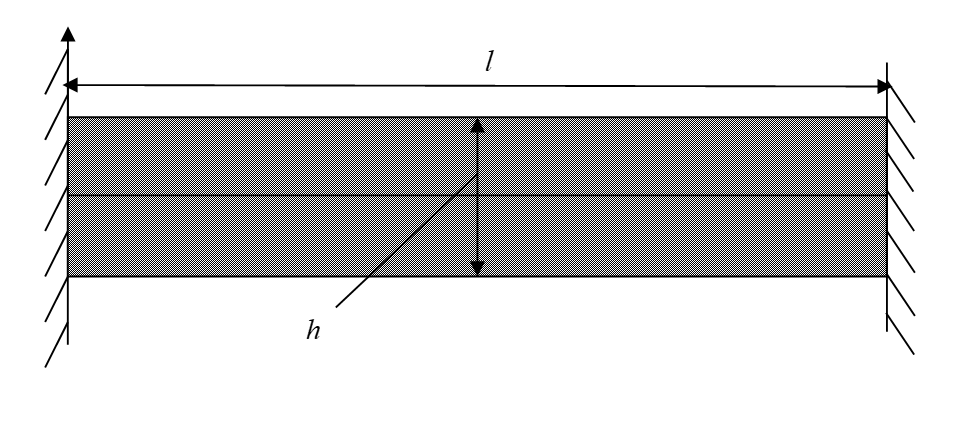
\includegraphics[scale=0.3]{pic/plate.png}
		\caption{Пластина-смуга з защемленими краями}
		\label{fig:plate}
\end{figure}



\end{frame}

\begin{frame}{Розділ 4}

\textbf{\textit{Лінійні коливання}}
\begin{figure}
	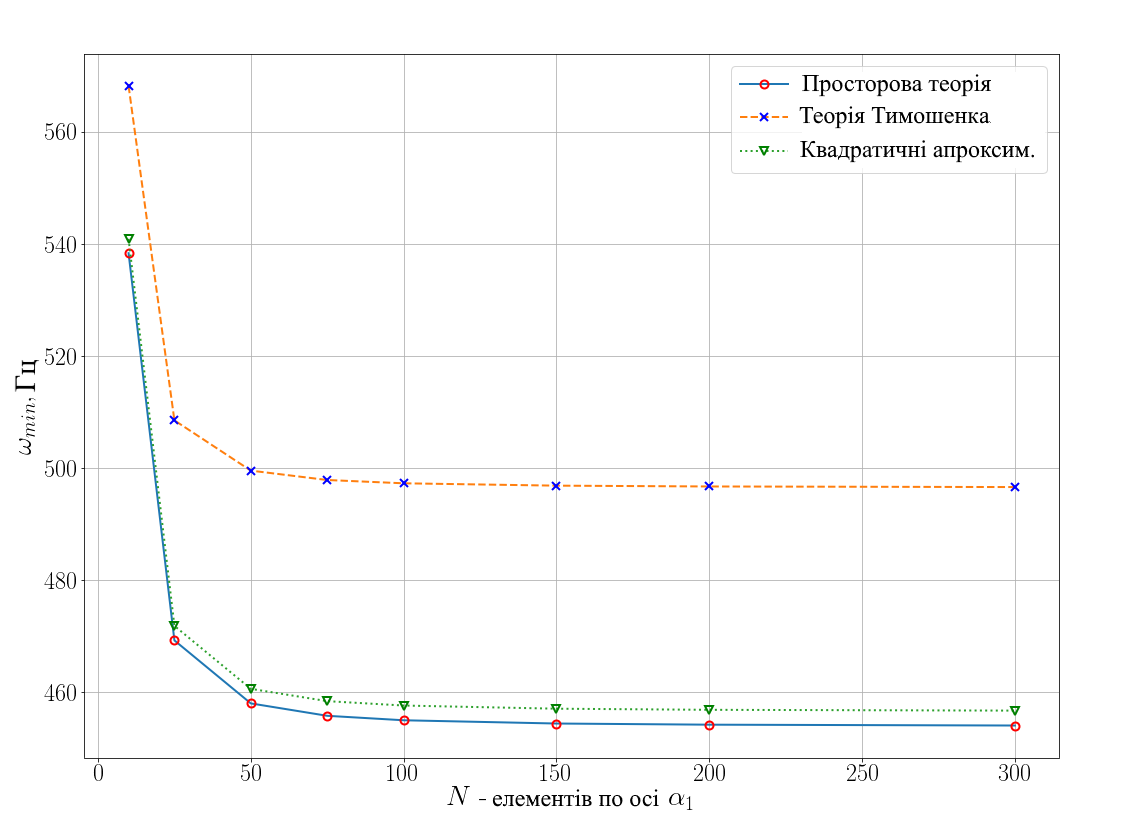
\includegraphics[scale=0.3]{pic/conv_allukr2.png}
		\caption{Збіжність процесу відшукання значення мінімальної власної частоти при збільшенні кількості скінченних елементів вздовж осі $\alpha_3$ для різних лінійних моделей.}
		\label{fig:EE31}
\end{figure}

\end{frame}


\begin{frame}{Розділ 4}

\textbf{\textit{Геометрично нелінійні коливання}}
\\
\vspace{1em}
З \eqref{eq:Kmatrix} і \eqref{eq:omega_nonlin}
\begin{equation}
\omega^2=\omega_0^2\left(1+\frac{3}{4}X\left(\frac{w_{max}}{h}\right)^2\right)
\end{equation}

\begin{tabbing}
де \= $\omega_0^2$ --- лінійна власна частота,\\
\> $\omega^2$ --- нелінійна власна частота.
\end{tabbing}

\begin{equation}
X=\frac{\overline{\phi}^T K_{NL}^{(2)}\left( h\overline{\phi}',h\overline{\phi}' \right) \overline{\phi}}{\omega_0^2}
\end{equation}

\begin{tabbing}
де \= $\overline{\phi}'$ --- нормований власний вектор $\overline{\phi}$.
\end{tabbing}


%\end{frame}
%
%\begin{frame}{Розділ 4}
\begin{table}[h!]
\caption{Значення параметра $X$ для різних моделей панелі, видовжені краї якої защемлені}
\centering
 \begin{tabular}{| l | c |} 
 \hline
 & $X$ \\ 
 \hline
 Аналітичне значення\footnotemark & 0.8363 \\ 
 \hline
 Зсувна модель Тимошенко & 0.8694 \\ 
 \hline
 Модель на основі квадратичних апроксимацій & 1.4586 \\ 
 \hline
 Модель на основі просторової теорії & 3.2488 \\
 \hline
\end{tabular}
\end{table}


\footnotetext[1]{Marchuk M., Pakosh V., Lesyk O., Hurayewska I. Influence of Pliability to Transversal Deformations of Shear and Compression on Correlation Frequency from Amplitude for Nonlinear Oscillations of Composite Plates // Vibrations in Physical Systems. - 2006. - Vol. XXII. - P. 251-256.}

\end{frame}




\begin{frame}{Розділ 4}

\begin{figure}
	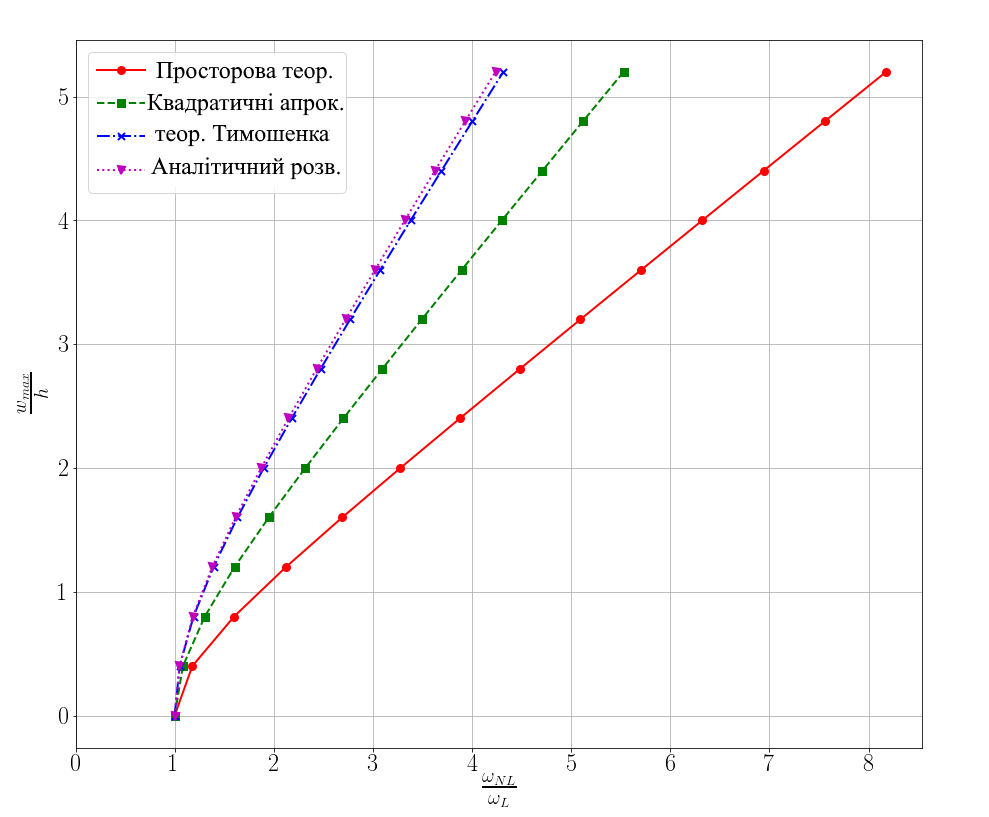
\includegraphics[scale=0.3]{pic/AFRC1ukr2.png}
		\caption{Амплітудно-частотні характеристики, отримані за допомогою узагальненого методу збурень для панелі, видовжені краї якої защемлені}
		\label{fig:AFR_C}
\end{figure}


\end{frame}

\begin{frame}{Розділ 4}
\textbf{Тришарова пластина-смуга}

\begin{figure}
	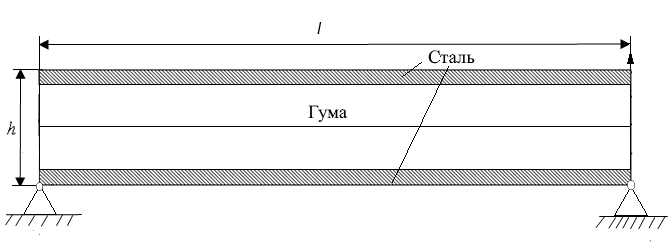
\includegraphics[scale=0.4]{pic/plate3layers_ukr.png}
		\caption{Тришарова пластина-смуга з нерухомими шарнірами на видовжених краях}
\end{figure}

Умови контакту між шарами
\begin{gather}
u_i^{(k-1)}\left(\alpha_1, h_{k-1},t \right)=u_i^{(k)}\left(\alpha_1, h_{k},t \right),\\
S^{(k-1)3i}\left(\alpha_1, h_{k-1},t \right)=S^{(k)3i}\left(\alpha_1, h_{k},t \right),
\end{gather}
\[ i=1,3, \alpha_1 \in [0;L], k=2,\dots,N.\]
Граничні умови на лицевих площинах панелі
\begin{equation}
S^{(m)31}\left(\alpha_1, h_{m},t \right)=S^{(m)33}\left(\alpha_1, h_{m},t \right)=0,\alpha_1 \in [0;L], m=0,N.
\end{equation}

\end{frame}


\begin{frame}{Розділ 4}
Геометричні та фізико-механічні характеристики
\begin{equation}
\begin{gathered}
L=1\text{м}, h=0.1\text{м};\\
\text{Сталь:}\qquad
E_1=E_3=210\cdot 10^{9} Па, v_{13}=v_{31}=0.3, \rho=8000 кг/м^3;\\
\text{Гума:}\qquad
E_1=E_3=0.1\cdot 10^{9} Па, v_{13}=v_{31}=0.48, \rho=1200 кг/м^3.
\end{gathered}
\end{equation}

\begin{table}[h!]
\caption{Вплив товщини шару гуми ($h_{r}$) на мінімальну власну частоту}
\centering
 \begin{tabular}{| c | c | c | c | c | c | c | c |} 
 \hline
 $\displaystyle \frac{h_{r}}{h}$ & 1 & 0.95 & 0.9 & 0.8 & 0.6 & 0.4 & 0 \\ 
  \hline
 $\omega_0$, Гц & 25.061 & 72.121 & 69.587 & 69.056 & 84.453 & 111.765 & 375.763 \\
   \hline
\end{tabular}
\end{table}

\begin{table}[h!]
\caption{Вплив товщини шару гуми ($h_{r}$) на значення параметра нелінійності $X$}
\centering
 \begin{tabular}{| c | c | c | c | c | c | c | c |} 
 \hline
 $\displaystyle \frac{h_{r}}{h}$ & 1 & 0.95 & 0.9 & 0.8 & 0.6 & 0.4 & 0 \\ 
  \hline
 $X$ & 16.1053 & 44.0470 & 73.2043 & 104.7005 & 92.1796 & 59.2721 & 5.7266 \\
   \hline
\end{tabular}
\end{table}

\end{frame}

\begin{frame}{Розділ 4}

\begin{figure}
	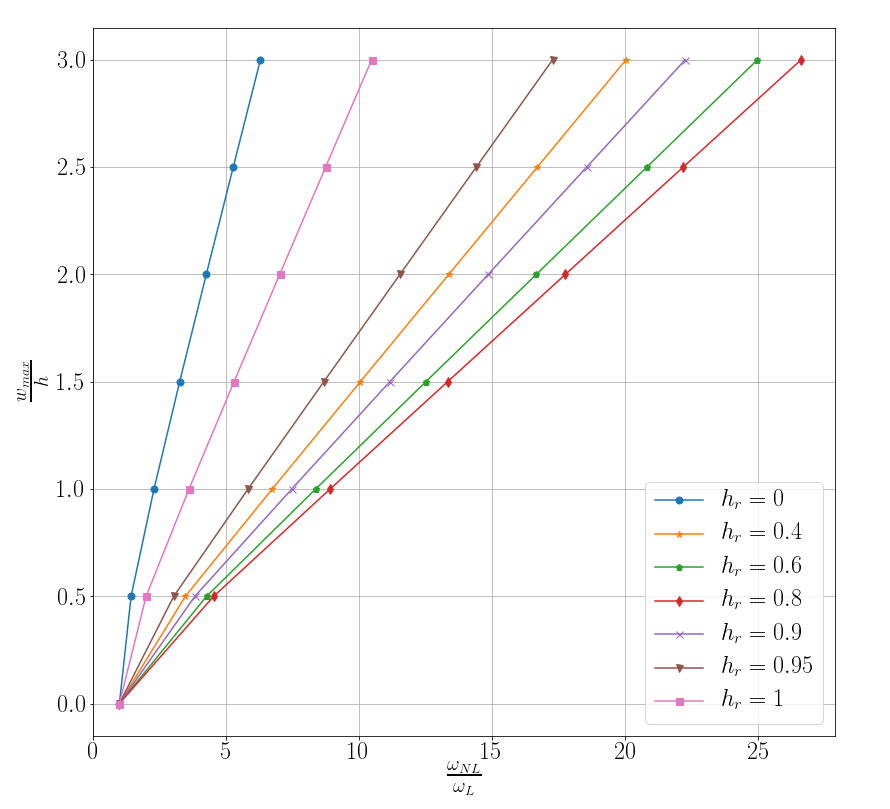
\includegraphics[scale=0.2]{pic/AFR_layered2.png}
		\caption{Амплітудно-частотні характеристики для тришарової панелі з нерухомими шарнірами на видовжених краях для різних значень $h_{r}$}
		\label{fig:AFR_layers}
\end{figure}


\end{frame}

\begin{frame}{Розділ 4}
\textbf{Видовжена циліндрична панель}
\begin{equation}
A\left( \alpha_1 \right)=1, \quad K\left( \alpha_1 \right)=\frac{1}{R}.
\end{equation}
Геометричні та фізико-механічні характеристики
\begin{equation}
\begin{gathered}
l=1\text{м}, h=0.01\text{м},\\
E_1=40E_3, v_{13}=v_{31}=0.25, G_{13}=0.6E_3.
\end{gathered}
\end{equation}

\begin{figure}
	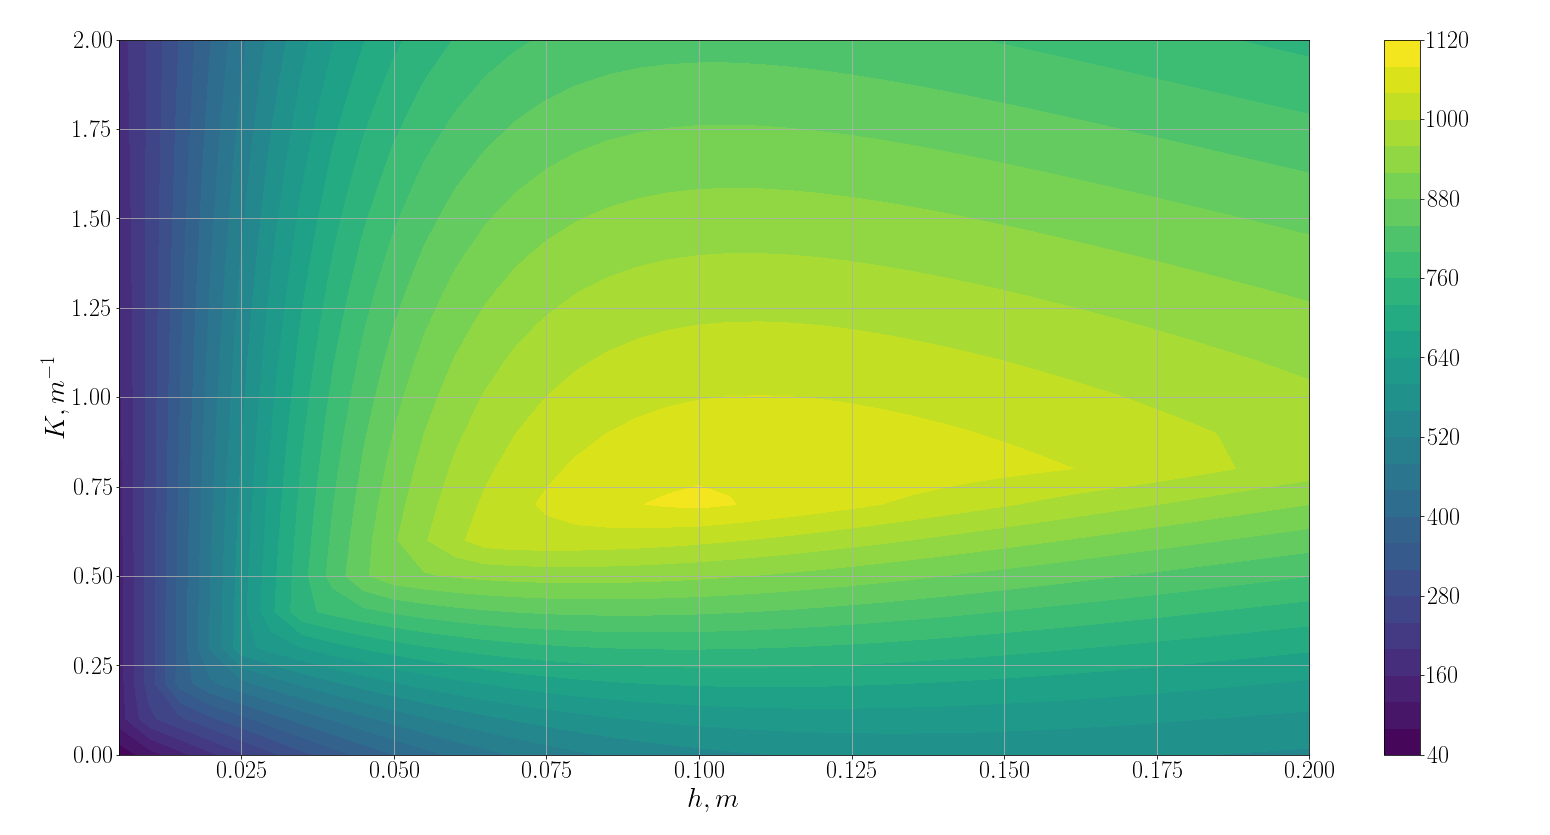
\includegraphics[scale=0.17]{pic/thickness_curvature_contour_plot2.png}
		\caption{Залежність найменшої власної частоти ($\omega_0$) від радіуса кривини $K$ і товщини $h$ циліндричної панелі}
		\label{fig:omaga_K_h}
\end{figure}
\end{frame}

\begin{frame}{Розділ 4}
\begin{table}[h!]
\caption{Вплив кривини напрямної ($K$) на значення параметра $X$}
\centering
 \begin{tabular}{| c | c | c | c | c | c |} 
 \hline
 $K, м^{-1}$ & 0.5 & 0.8 & 1 & 1.5 & 2 \\ 
  \hline
 $X$ & 4.442 & 4.203 & 4.002 & 3.421 & 2.855 \\
   \hline
\end{tabular}
\end{table}

\begin{figure}
	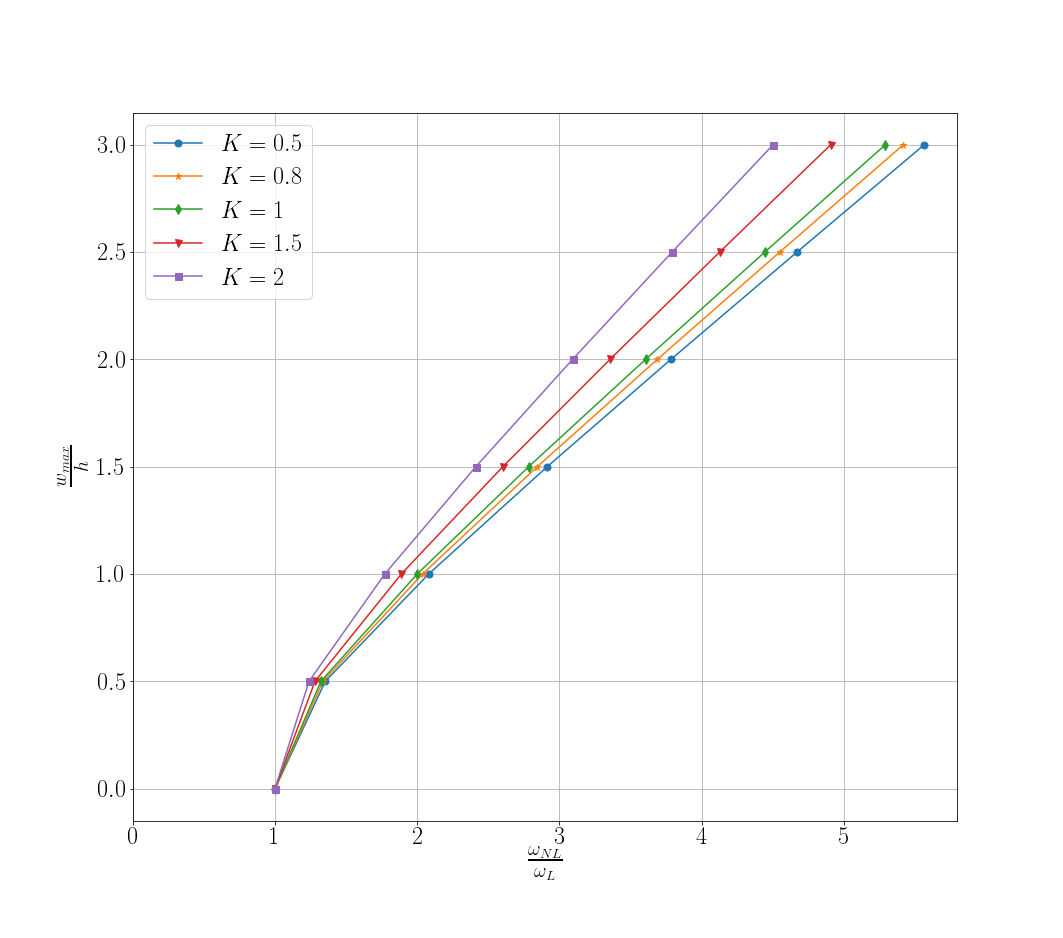
\includegraphics[scale=0.2]{pic/AFR_curvature.png}
		\caption{Амплітудно-частотні характеристики для панелі з вуглепластика з для різних значень кривини напрямної $K$}
		\label{fig:AFR_layers}
\end{figure}

\end{frame}

\section{РОЗДІЛ 5}

\begin{frame}{РОЗДІЛ 5. ВІЛЬНІ КОЛИВАННЯ ГОФРОВАНИХ ЦИЛІНДРИЧНИХ ОБОЛОНОК}
\textbf{Геометричні співвідношення і базові вектори для гофрованої циліндричної оболонки}
\\
\begin{equation}
\begin{aligned}
x_1&=\left(R + g_{A}\cos\left(g_v\theta\right) \right)\cos\left(\theta\right), \\
x_2&=\alpha_2,\\
x_3&=\left(R + g_{A}\cos\left(g_v\theta\right) \right)\sin\left(\theta\right), 
\end{aligned}
\end{equation}

\begin{tabbing}
де \= $L$ --- довжина напрямної циліндричної оболонки,\\
\> $R$ --- відстань від осі панелі до напрямної циліндричної оболонки,\\
\> $h$ --- товщина гофрованої оболонки,\\
\> $g_A$ --- амплітуда гофрування,\\
\> $g_v$ --- частота гофрування,\\
\end{tabbing}
\[
\theta=\theta\left(\alpha_1\right)=\frac{\pi}{2}+\frac{1}{R}\left(\frac{L}{2}-\alpha_1\right)\]

Коефіцієнт першої квадратичної форми і головна кривина 
\begin{gather}
A\left(\alpha_1\right) = \sqrt{w^2+z^2},
K\left(\alpha_1\right) = \frac{\left(wy+2z^2/R\right)}{A\left(\alpha_1\right)^{\frac{3}{2}}},
\end{gather}
де
\begin{gather*}
w=1+\frac{g_A}{R}\cos\left(g_v\theta\right),
z=\frac{g_A g_v}{R}\sin\left(g_v\theta\right),
y=-\frac{w}{R}+\frac{g_A g_v^2}{R^2}\cos\left(g_v\theta\right).
\end{gather*}

\end{frame}


\begin{frame}{Розділ 5}
\begin{figure}
	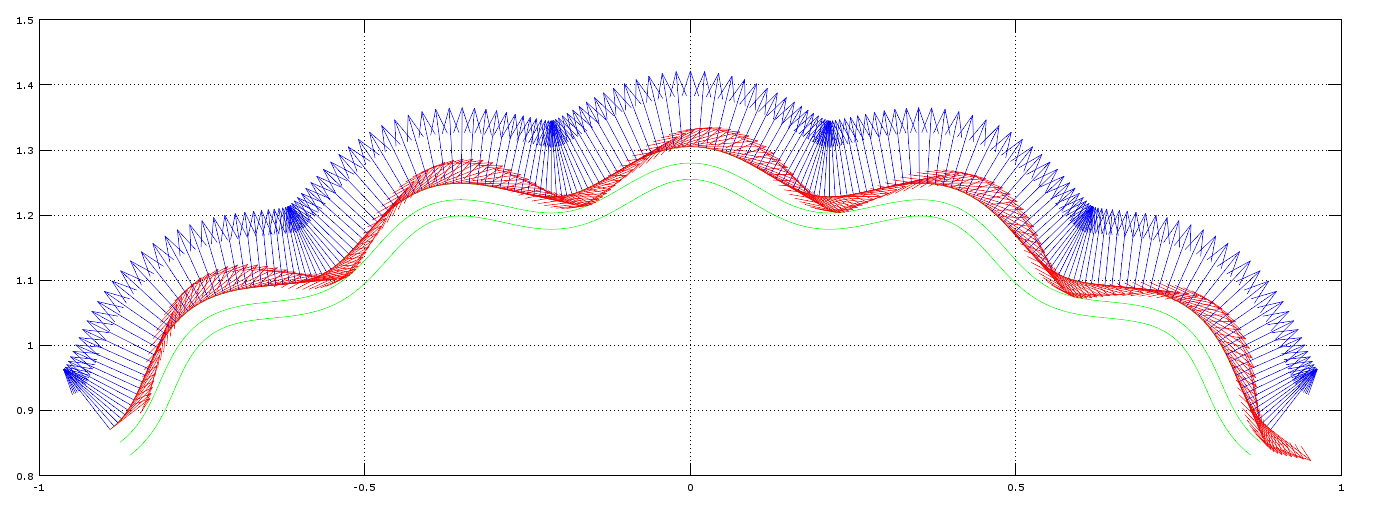
\includegraphics[scale=0.2]{pic/cor_R1R32.png}
		\caption{Вектори коваріантної бази $\vec{R}_1$ (червоний колір) і $\vec{R}_3$ (синій колір) на верхній лицевій поверхні оболонки}
\end{figure}
Геометричні та фізико-механічні  характеристики
\begin{equation}
\begin{gathered}
L=2\text{м}, h=0.05\text{м},R=1.25\text{м},g_A=0.03\text{м}, g_v=20,\\
E_1=E_3=2.1\cdot 10^{11} Па, v_{13}=v_{31}=0.3, G_{13}=8.1\cdot 10^{10} Па,\\ \rho=8000 кг/м^3.
\end{gathered}
\end{equation}
\end{frame}

\begin{frame}{Розділ 5}
\textbf{Лінійні коливання}
\\
\begin{table}[h!]
\caption{Залежність найменшої власної частоти ($\omega_0$) від частоти гофрування ($g_v$) оболонки}
\centering
%\resizebox{\textwidth}{!}{
 \begin{tabular}{| c | c | c | c | c | c | c | c | c | c | c | c | c | c | c |} 
 \hline
 $g_v$ & 2 & 4 & 6 & 8 & 15 & 20 & 50 \\ 
  \hline
 $\omega_0$, Гц & 105 & 98 & 92 & 110 & 132 & 217 & 2588\\
   \hline
\end{tabular}%}
\end{table}

\begin{table}[h!]
\caption{Залежність найменшої власної частоти ($\omega_0$) від амплітуди гофрування ($g_A$) оболонки}
\centering
 \begin{tabular}{| c | c | c | c | c | c | c | c | c |} 
 \hline
 $g_A$, м & 0 & 0.015 & 0.03 & 0.06 & 0.1 & 0.2 & 0.25 & 0.3 \\ 
  \hline
 $\omega_0$, Гц & 101 & 143 & 217 & 377 & 622 & 675 & 552 & 461\\
   \hline
\end{tabular}
\end{table}

\begin{figure}[h]
\begin{minipage}[h]{0.49\linewidth}
\center{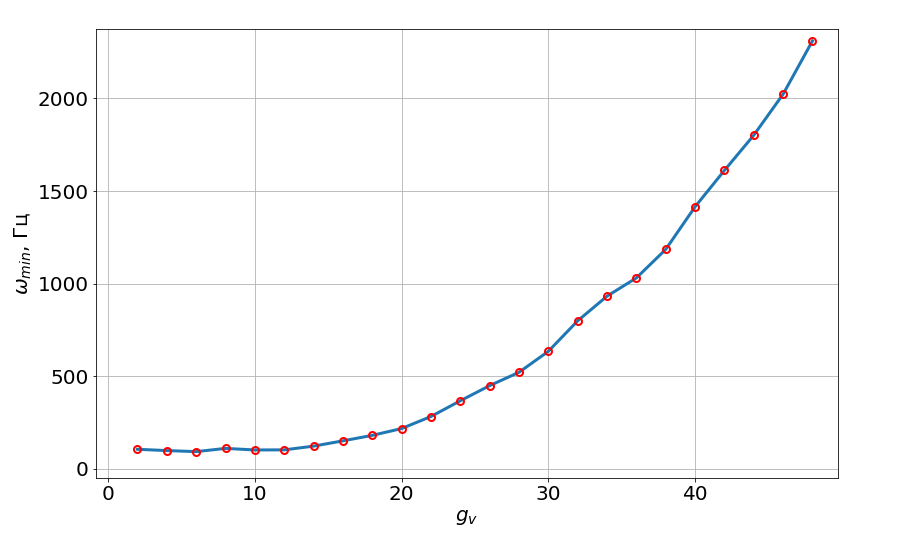
\includegraphics[width=0.9\linewidth]{pic/gv_freq2.png} \\ а)}
\end{minipage}
\hfill
\begin{minipage}[h]{0.49\linewidth}
\center{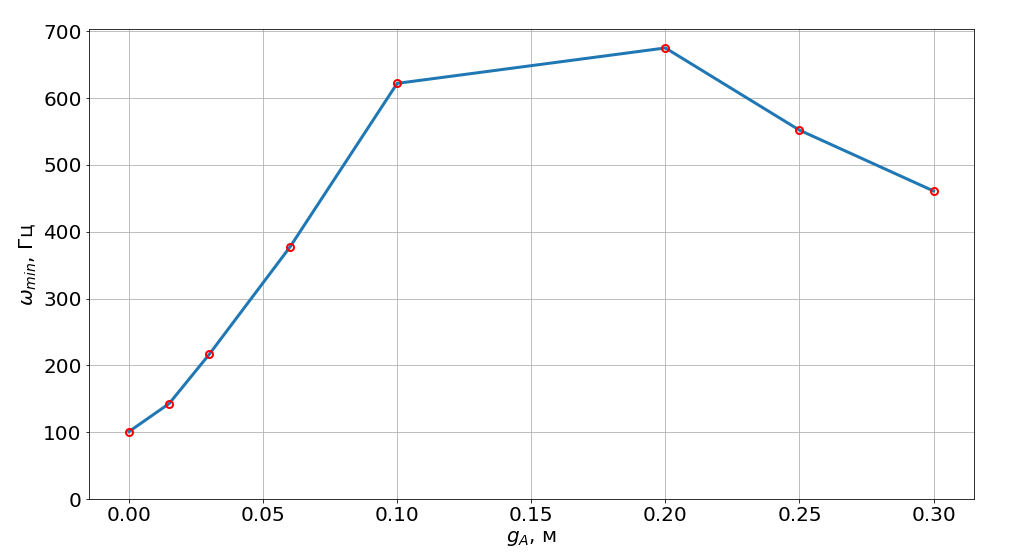
\includegraphics[width=0.9\linewidth]{pic/corrugated_ampl_linear.png} \\ б)}
\end{minipage}
\caption{Залежність найменшої власної частоти ($\omega_0$) від: \\а) частоти гофрування ($g_v$) б) амплітуди гофрування ($g_A$) оболонки}
\end{figure}
\end{frame}


\begin{frame}{Розділ 5}
\begin{figure}[h]
\begin{minipage}[h]{0.49\linewidth}
\center{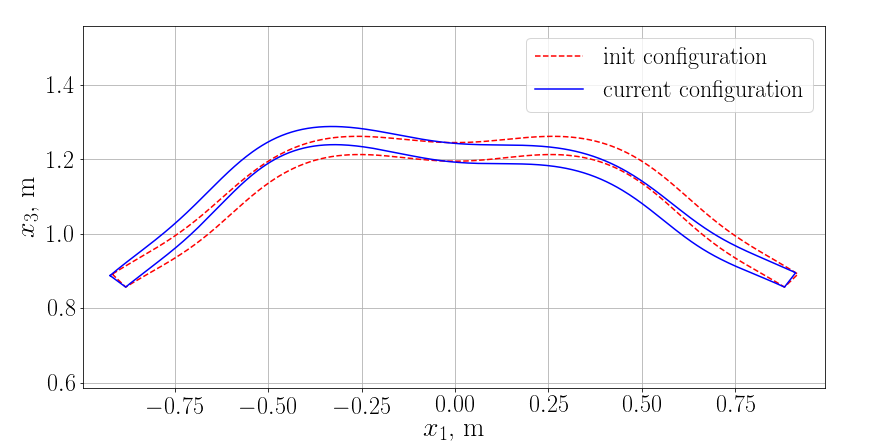
\includegraphics[width=\linewidth]{pic/corrugated_deforms_10.png} \\ а)}
\end{minipage}
\hfill
\begin{minipage}[h]{0.49\linewidth}
\center{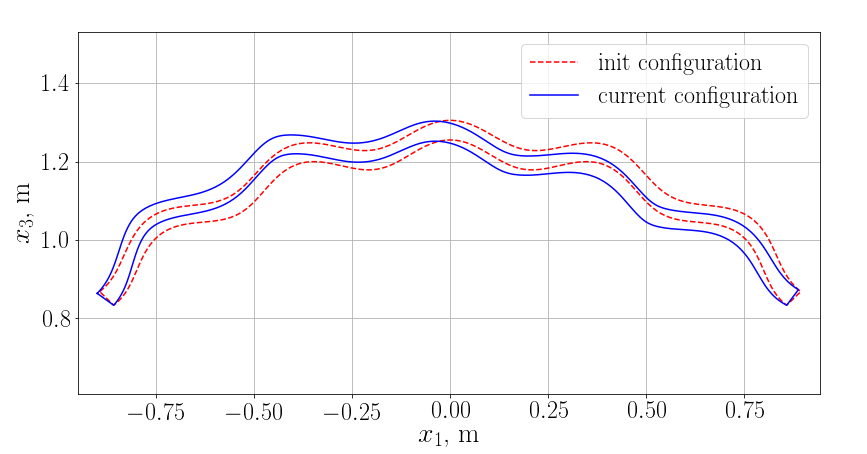
\includegraphics[width=\linewidth]{pic/corrugated_deforms_20.png} \\ б)}
\end{minipage}
\caption{Перша мода гофрованої циліндричної панелі з різними частотами гофрування: а) $g_v=10$; б)$g_v=20$.}
\end{figure}

\begin{figure}[h]
\begin{minipage}[h]{0.49\linewidth}
\center{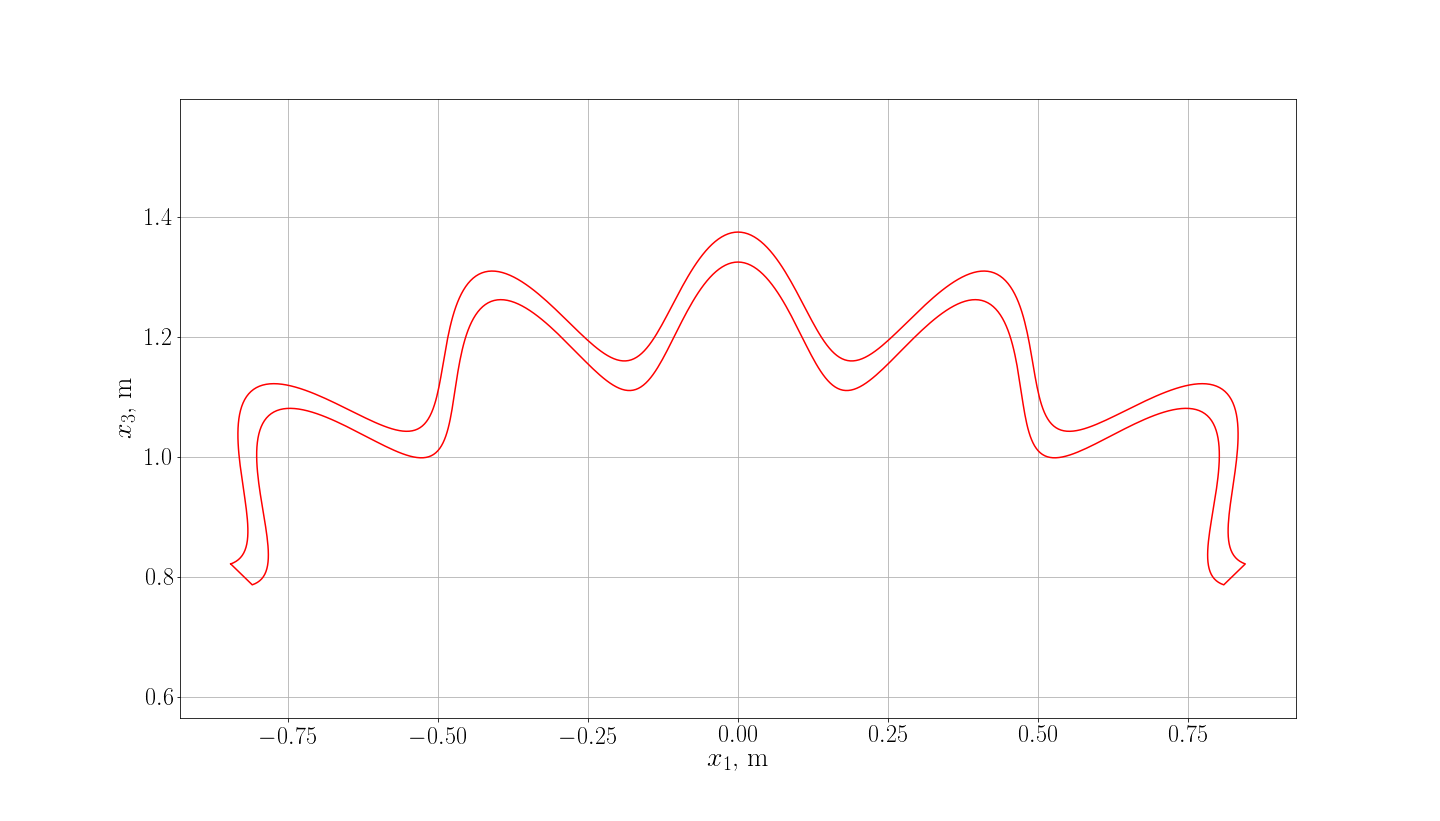
\includegraphics[width=\linewidth]{pic/cor_geom_ga01.png} \\ а)}
\end{minipage}
\hfill
\begin{minipage}[h]{0.49\linewidth}
\center{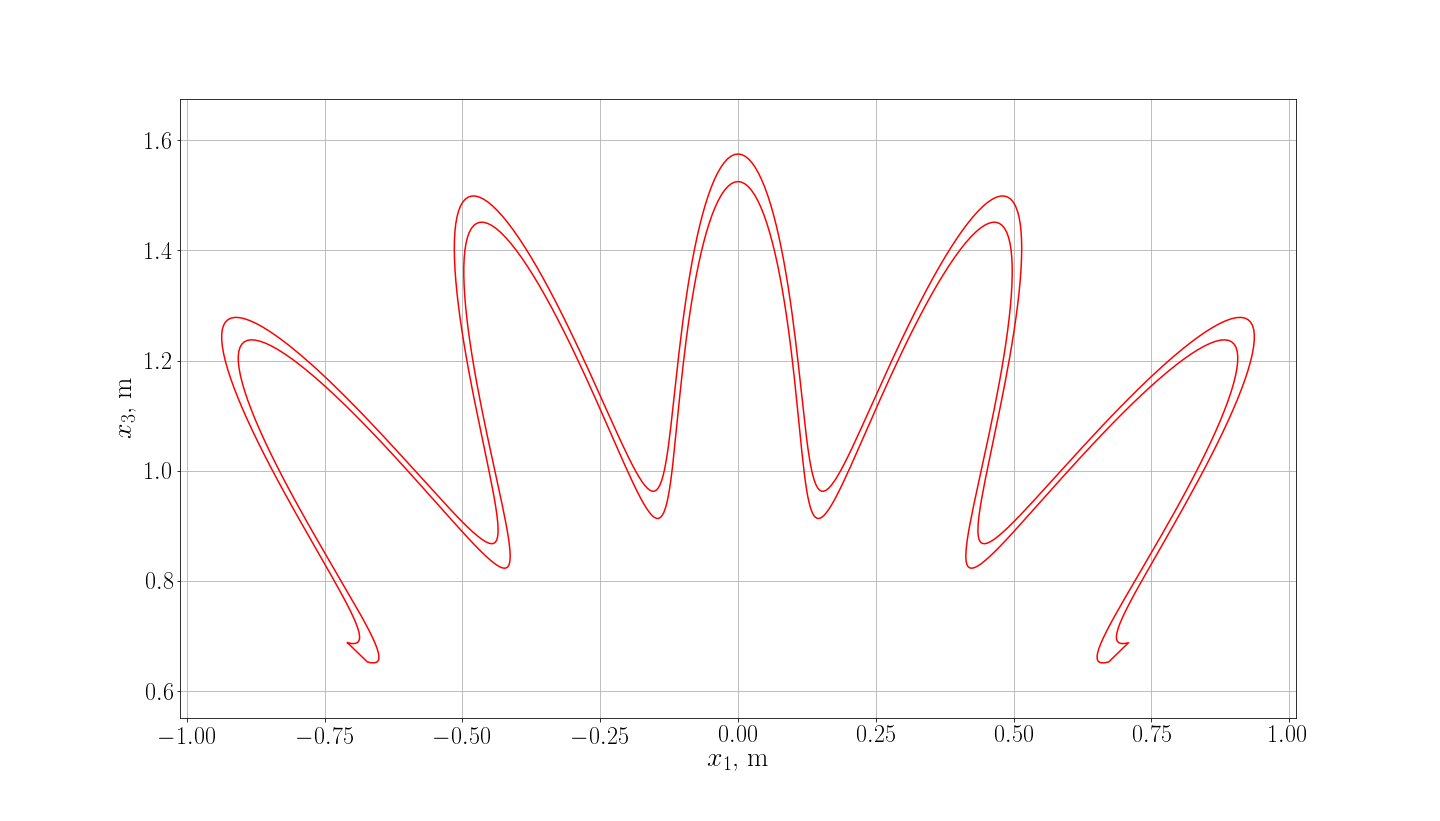
\includegraphics[width=\linewidth]{pic/cor_geom_ga03.png} \\ б)}
\end{minipage}
\caption{Вигляд гофрованої циліндричної панелі при a) $g_A = 0.1м$; б) $g_A = 0.3м$.}
\end{figure}
\end{frame}


\begin{frame}{Розділ 5}
\textbf{Геометрично нелінійні коливання}
\begin{table}[h!]
\caption{Вплив частоти гофрування ($g_v$) на значення параметра $X$}
\centering
 \begin{tabular}{| c | c | c | c | c | c |} 
 \hline
 $g_v$ & 2 & 6 & 15 & 20 & 50 \\ 
  \hline
 $X$ & 6.6324 & 7.5217 & 2.9688 & 1.2465 & 0.0728 \\
   \hline
\end{tabular}
\end{table}
\begin{table}[h!]
\caption{Вплив амплітуди гофрування ($g_A$) на значення параметра $X$}
\centering
 \begin{tabular}{| c | c | c | c | c | c | c |} 
 \hline
 $g_A, м$ & 0 & 0.03 & 0.1 & 0.2 & 0.25 & 0.3 \\ 
  \hline
 $X$ & 6.5853 & 1.2465 & 0.0815 & 2.4986 & 7.5377 & 40.1717 \\
   \hline
\end{tabular}
\end{table}
\begin{figure}[h]
\begin{minipage}[h]{0.49\linewidth}
\center{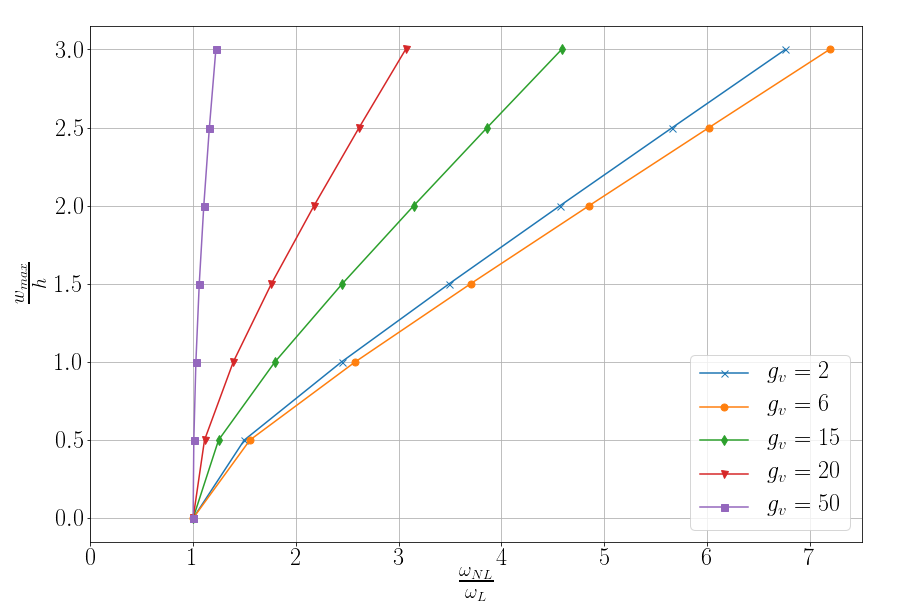
\includegraphics[width=0.9\linewidth]{pic/corrugated_nonlinear.png} \\ а)}
\end{minipage}
\hfill
\begin{minipage}[h]{0.49\linewidth}
\center{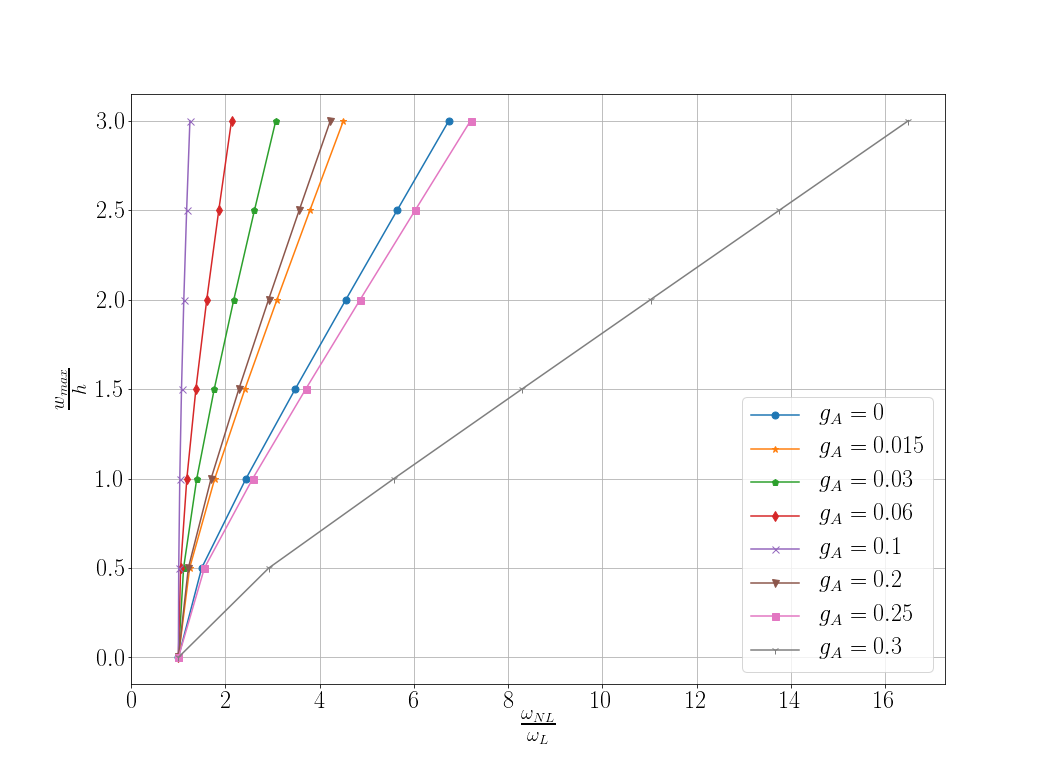
\includegraphics[width=0.9\linewidth]{pic/corrugated_ampl_nonlinear_s.png} \\ б)}
\end{minipage}
\caption{Амплітудно-частотні характеристики гофрованої оболонки: \\а) для різних значень частоти гофрувань ($g_v$); б) для різних значень амплітуди гофрування ($g_A$)}
\end{figure}
\end{frame}


\section{ВИСНОВКИ}
\begin{frame}
\textbf{\large ВИСНОВКИ}
\\
\vspace{0.2em}
У дисертаційній роботі вирішено науково практичне завдання визначення амплітудо-частотних характеристик шаруватих пластин і гофрованих у коловому напрямку циліндричних оболонок. При цьому отриматі наступні результати:
\begin{itemize}
\item Побудовано нову модель геометрично нелінійного деформування видовжених циліндричних оболонок на основі квадратичних апроксимацій компонент вектора переміщень за нормальною координатою до серединної поверхні шару та показано її ефективність.
\item Узагальнено метод збурень для розв'язування систем нелінійних алгебричних рівнянь, які отримуються у задачах визначення амплітудно-частотних характеристик пластин і оболонок за геометрично нелінійного деформування.
\item Розроблено нову методику знаходження розв’язку задачі про вільні коливання за геометрично нелінійного деформування на основі методу скінченних елементів і методу збурення. Показано її ефективність шляхом порівняння з розв'язками, отриманими іншими авторами.
\end{itemize}
\end{frame}
\begin{frame}
\textbf{\large ВИСНОВКИ}
\\
\vspace{1em}
\begin{itemize}
\item Досліджено лінійні та геометрично нелінійні коливання тришарових пластин-смуг, які складаються з двох металевих лицевих та гумового середнього шарів.  Встановлено кількісний вплив товщини гумового шару на мінімальну власну частоту за лінійного та геометрично нелінійного деформування, а також визначено співвідношення між товщинами шарів, при якому вона досягає максимального значення. 
\item Проаналізовано лінійні та геометрично нелінійні коливання видовжених циліндричних панелей. Встановлено характер впливу кривини панелей та типу коливань на їхню жорсткість. 
\item Сформульовано постановки задач про лінійні та геометрично нелінійні коливання гофрованої циліндричної оболонки на основі використання співвідношень просторових теорій пружності. Встановлено вплив частоти та амплітуди гофрування оболонки на її жорсткість. Виявлено інтервали зростання та спадання першої власної частоти видовженої гофрованої циліндричної панелі за геометрично нелінійного деформування.

\end{itemize}



\end{frame}

\begin{frame}
\begin{center}
\Huge ДЯКУЮ ЗА УВАГУ!
\end{center}
\end{frame}
\end{document}